\chapter{Especificação/Análise da Aplicação}

\section{Formato de especificação}

\begin{table}[ht]
	\centering
	\resizebox{\textwidth}{!}{%
		\begin{tabular}{|c|c|c|c|}
			\hline
			\multirow{2}{*}{\textbf{Critério}} & \multicolumn{3}{c|}{\textbf{Formato de Especificação}} \\ \cline{2-4} 
			                                       & \textbf{Casos de Uso}     & \textbf{Casos de Uso 2.0}             & \textbf{Histórias de Usuário}    \\ \hline
															                        
			\multirow{2}{*}{\textbf{Quando Usar}}  & Projetos que necessitam   & Quando você precisa de um            & Desenvolvimento Ágil,             \\
			                                       & de uma visão abrangente  & formato estruturado e iterativo,      & projetos menores a médios,        \\
			                                       & e detalhada do sistema.   & adaptável a mudanças.               & ou quando o foco está nas         \\
			                                       &                           &                                       & necessidades do usuário final.    \\ \hline
															                        
			\multirow{4}{*}{\textbf{Benefícios}}  & Oferece alto nível de    & Oferece uma estrutura                 & Simples, focado,                   \\
			                                       & detalhamento e uma visão & detalhada, é iterativo,              & altamente adaptável a mudanças,  \\
			                                       & abrangente do sistema.    & flexível e adaptável.               & fácil de aprender e usar,         \\
			                                       &                           &                                       & e com baixo custo de manutenção. \\ \hline
															                        
			\multirow{4}{*}{\textbf{Desvantagens}} & Pode ser complexo e       & Requer planejamento cuidadoso         & Pode ser simplista                 \\
			                                       & demorado para desenvolver & e tem custo de manutenção moderado. & para funcionalidades complexas.    \\
			                                       & e manter. Ideal para      &                                       &                                    \\
			                                       & sistemas maiores.         &                                       &                                    \\ \hline
		\end{tabular}%
	}
	\caption{Comparação revisada entre Casos de Uso, Casos de Uso 2.0 e Histórias de Usuário}
	\label{tab:revised_comparison}
\end{table}

O projeto \textit{Fintrackr}, embora seja de pequeno porte, tem uma complexidade inerente que demanda uma visão mais detalhada e estruturada do sistema. Neste cenário, os \textit{Casos de Uso} surgem como o formato de especificação ideal. A abordagem de Casos de Uso permite uma representação mais profunda das interações do sistema, alinhando-se perfeitamente com a Clean Architecture ao focar nas interações e nos fluxos de negócios.

Os Casos de Uso oferecem uma representação clara das funções e interações do sistema, facilitando a comunicação entre desenvolvedores, stakeholders e usuários. Esta abordagem detalhada garante que todas as nuances e requisitos do \textit{Fintrackr} sejam capturados e desenvolvidos de forma eficaz. Ao adotar Casos de Uso, garantimos uma compreensão profunda das necessidades do usuário e uma implementação sistemática dessas necessidades.           

\section{Ferramentas de ALM}

\begin{table}[ht]
	\centering
	\resizebox{\textwidth}{!}{%
		\begin{tabular}{|c|c|c|c|c|c|}
			\hline
			\multirow{2}{*}{\textbf{Critério}} & \multicolumn{5}{c|}{\textbf{Ferramenta}} \\ \cline{2-6} 
			                                       & \textbf{Jira}             & \textbf{Trello}        & \textbf{Tuleap}         & \textbf{GitLab}           & \textbf{Notion}              \\ \hline
												                        
			\multirow{2}{*}{\textbf{Quando Usar}}  & Projetos ágeis,          & Projetos simples,      & Desenvolvimento ágil,  & Desenvolvimento e         & Geração e controle de      \\
			                                       & de médio a grande porte. & visualização Kanban. & integração contínua. & integração contínua.   & tarefas, visões múltiplas. \\ 
			                                       &                           &                        & projetos open source.   &                           & do mesmo datasource.         \\ \hline
												                        
			\multirow{4}{*}{\textbf{Benefícios}}  & Flexível, integrações  & Simples, intuitivo,    & Open source,            & Integração contínua,   & Facilidade na geração e    \\
			                                       & amplas, poderoso.         & flexível.             & personalizável.        & gestão de código.       & controle de tarefas.         \\
			                                       &                           &                        &                         & gerenciamento de projeto. &                              \\
			                                       &                           &                        &                         &                           &                              \\ \hline
												                        
			\multirow{4}{*}{\textbf{Desvantagens}} & Curva de aprendizado      & Pode ser simplista     & Pode ser complexo       & Pode ser sobrecarregado   & -                            \\
			                                       & íngreme, pode ser caro.  & para grandes projetos. & para novatos.           & para projetos menores.    &                              \\
			                                       &                           &                        &                         &                           &                              \\ 
			                                       &                           &                        &                         &                           &                              \\ \hline
		\end{tabular}%
	}
	\caption{Comparação entre Jira, Trello, Tuleap, GitLab e Notion}
	\label{tab:tool_comparison}
\end{table}          
        

Dada a natureza do projeto \textit{Fintrackr}, a seleção de ferramentas para gerenciamento e desenvolvimento é crucial. Optamos pelo Notion devido à sua facilidade na geração e controle de tarefas, permitindo várias visões diferentes do mesmo datasource. Além disso, o Notion também nos permite criar documentações detalhadas para nossos projetos. Complementando nossa escolha, adotamos um \href{https://github.com/ThiagoSchumann/fintrackr-docs}{repositório no GitHub} para centralizar outros aspectos da documentação e artefatos, oferecendo uma visão unificada do projeto. Essa combinação de Notion e GitHub é ideal para as necessidades do \textit{Fintrackr}.

\section{Planejamento do desenvolvimento}
            
\section{Backlog}

\begin{figure}[ht]
	\centering
	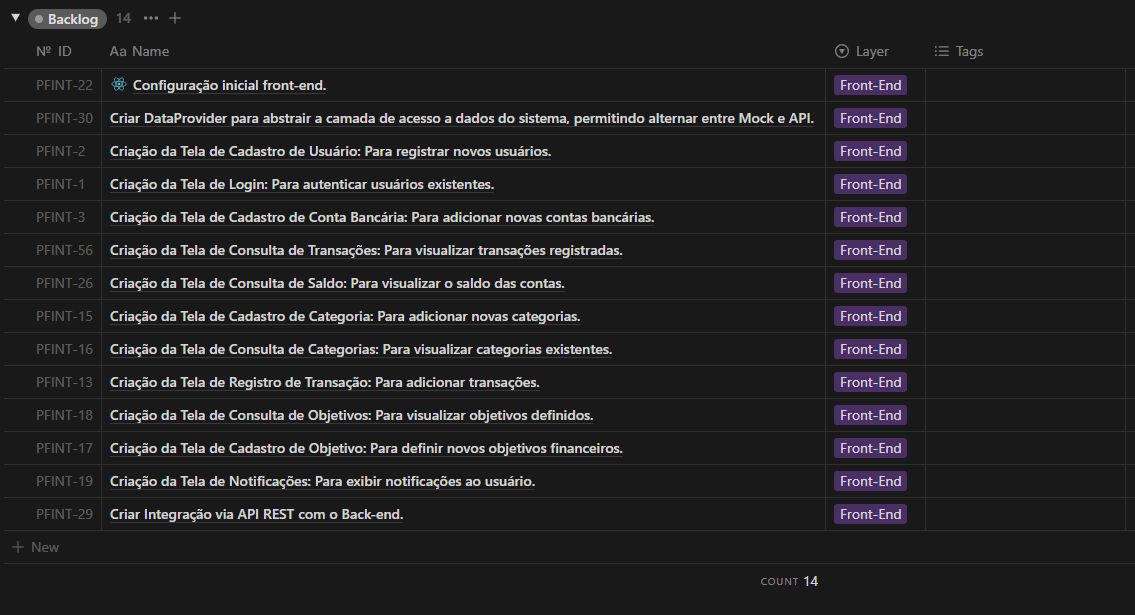
\includegraphics[width=1\linewidth]{Textuais/images/backlog-front-end.png}
	\caption{Backlog referente ao Front-end.}
	\label{fig:backlog-front-end}
\end{figure}

\begin{figure}[ht]
	\centering
	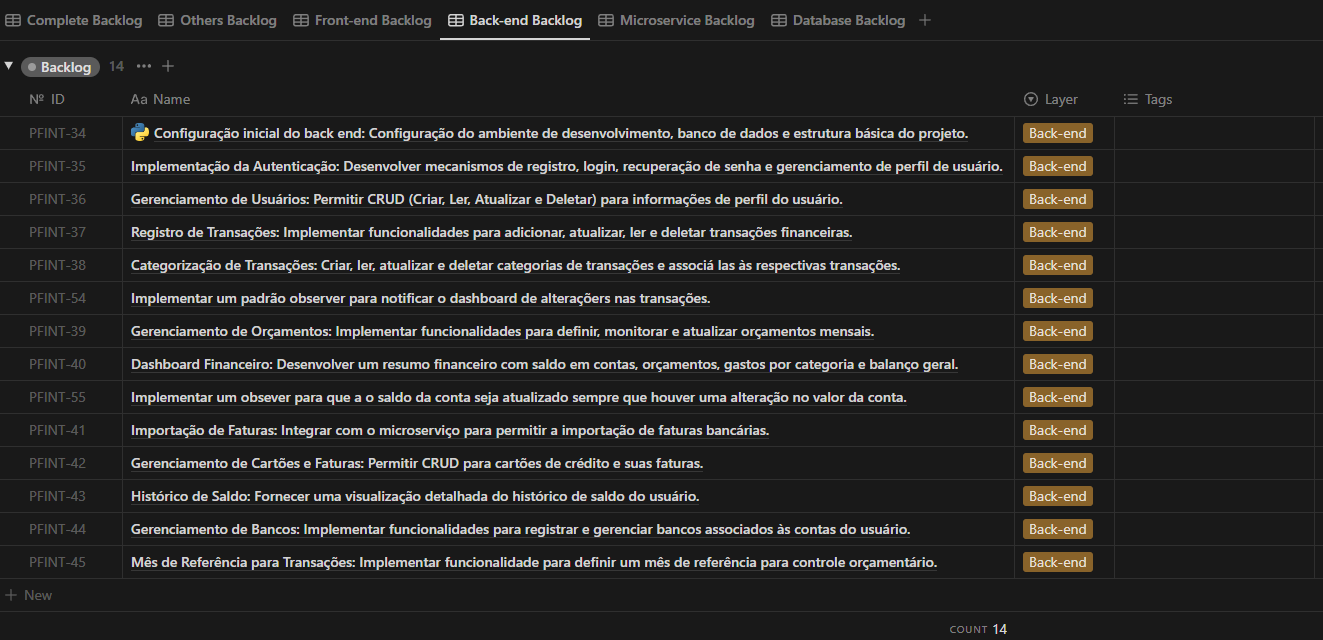
\includegraphics[width=1\linewidth]{Textuais/images/backlog-back-end.png}
	\caption{Backlog referente ao Back-end Principal.}
	\label{fig:backlog-back-end}
\end{figure}

\begin{figure}[ht]
	\centering
	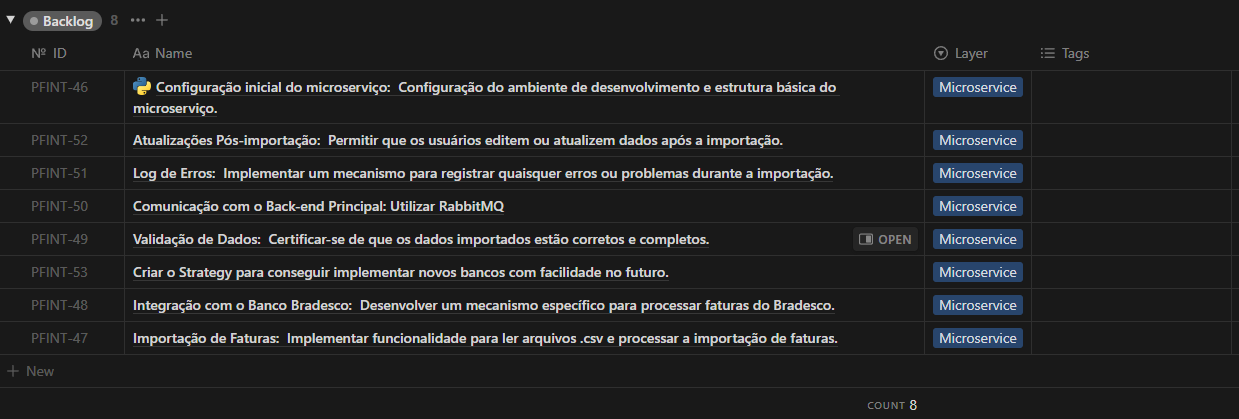
\includegraphics[width=1\linewidth]{Textuais/images/backlog-microservice.png}
	\caption{Backlog referente ao Microserviço.}
	\label{fig:backlog-microservice}
\end{figure}